\documentclass[twoside]{book}

% Packages required by doxygen
\usepackage{fixltx2e}
\usepackage{calc}
\usepackage{doxygen}
\usepackage[export]{adjustbox} % also loads graphicx
\usepackage{graphicx}
\usepackage[utf8]{inputenc}
\usepackage{makeidx}
\usepackage{multicol}
\usepackage{multirow}
\PassOptionsToPackage{warn}{textcomp}
\usepackage{textcomp}
\usepackage[nointegrals]{wasysym}
\usepackage[table]{xcolor}

% Font selection
\usepackage[T1]{fontenc}
\usepackage[scaled=.90]{helvet}
\usepackage{courier}
\usepackage{amssymb}
\usepackage{sectsty}
\renewcommand{\familydefault}{\sfdefault}
\allsectionsfont{%
  \fontseries{bc}\selectfont%
  \color{darkgray}%
}
\renewcommand{\DoxyLabelFont}{%
  \fontseries{bc}\selectfont%
  \color{darkgray}%
}
\newcommand{\+}{\discretionary{\mbox{\scriptsize$\hookleftarrow$}}{}{}}

% Page & text layout
\usepackage{geometry}
\geometry{%
  a4paper,%
  top=2.5cm,%
  bottom=2.5cm,%
  left=2.5cm,%
  right=2.5cm%
}
\tolerance=750
\hfuzz=15pt
\hbadness=750
\setlength{\emergencystretch}{15pt}
\setlength{\parindent}{0cm}
\setlength{\parskip}{0.2cm}
\makeatletter
\renewcommand{\paragraph}{%
  \@startsection{paragraph}{4}{0ex}{-1.0ex}{1.0ex}{%
    \normalfont\normalsize\bfseries\SS@parafont%
  }%
}
\renewcommand{\subparagraph}{%
  \@startsection{subparagraph}{5}{0ex}{-1.0ex}{1.0ex}{%
    \normalfont\normalsize\bfseries\SS@subparafont%
  }%
}
\makeatother

% Headers & footers
\usepackage{fancyhdr}
\pagestyle{fancyplain}
\fancyhead[LE]{\fancyplain{}{\bfseries\thepage}}
\fancyhead[CE]{\fancyplain{}{}}
\fancyhead[RE]{\fancyplain{}{\bfseries\leftmark}}
\fancyhead[LO]{\fancyplain{}{\bfseries\rightmark}}
\fancyhead[CO]{\fancyplain{}{}}
\fancyhead[RO]{\fancyplain{}{\bfseries\thepage}}
\fancyfoot[LE]{\fancyplain{}{}}
\fancyfoot[CE]{\fancyplain{}{}}
\fancyfoot[RE]{\fancyplain{}{\bfseries\scriptsize Generated on Fri Apr 10 2015 15\+:00\+:00 for Bubble Streamer by Doxygen }}
\fancyfoot[LO]{\fancyplain{}{\bfseries\scriptsize Generated on Fri Apr 10 2015 15\+:00\+:00 for Bubble Streamer by Doxygen }}
\fancyfoot[CO]{\fancyplain{}{}}
\fancyfoot[RO]{\fancyplain{}{}}
\renewcommand{\footrulewidth}{0.4pt}
\renewcommand{\chaptermark}[1]{%
  \markboth{#1}{}%
}
\renewcommand{\sectionmark}[1]{%
  \markright{\thesection\ #1}%
}

% Indices & bibliography
\usepackage{natbib}
\usepackage[titles]{tocloft}
\setcounter{tocdepth}{3}
\setcounter{secnumdepth}{5}
\makeindex

% Hyperlinks (required, but should be loaded last)
\usepackage{ifpdf}
\ifpdf
  \usepackage[pdftex,pagebackref=true]{hyperref}
\else
  \usepackage[ps2pdf,pagebackref=true]{hyperref}
\fi
\hypersetup{%
  colorlinks=true,%
  linkcolor=blue,%
  citecolor=blue,%
  unicode%
}

% Custom commands
\newcommand{\clearemptydoublepage}{%
  \newpage{\pagestyle{empty}\cleardoublepage}%
}


%===== C O N T E N T S =====

\begin{document}

% Titlepage & ToC
\hypersetup{pageanchor=false,
             bookmarks=true,
             bookmarksnumbered=true,
             pdfencoding=unicode
            }
\pagenumbering{roman}
\begin{titlepage}
\vspace*{7cm}
\begin{center}%
{\Large Bubble Streamer }\\
\vspace*{1cm}
{\large Generated by Doxygen 1.8.9.1}\\
\vspace*{0.5cm}
{\small Fri Apr 10 2015 15:00:00}\\
\end{center}
\end{titlepage}
\clearemptydoublepage
\tableofcontents
\clearemptydoublepage
\pagenumbering{arabic}
\hypersetup{pageanchor=true}

%--- Begin generated contents ---
\chapter{Hierarchical Index}
\section{Class Hierarchy}
This inheritance list is sorted roughly, but not completely, alphabetically\+:\begin{DoxyCompactList}
\item \contentsline{section}{Bubble}{\pageref{struct_bubble}}{}
\item \contentsline{section}{Bubble\+Agent}{\pageref{class_bubble_agent}}{}
\begin{DoxyCompactList}
\item \contentsline{section}{Disk}{\pageref{class_disk}}{}
\end{DoxyCompactList}
\item \contentsline{section}{Bubble\+Solver}{\pageref{class_bubble_solver}}{}
\item \contentsline{section}{Fluid\+Sim}{\pageref{class_fluid_sim}}{}
\item S\+O\+P\+\_\+\+Node\begin{DoxyCompactList}
\item \contentsline{section}{S\+O\+P\+\_\+\+Bubble\+Streamer}{\pageref{class_s_o_p___bubble_streamer}}{}
\end{DoxyCompactList}
\end{DoxyCompactList}

\chapter{Class Index}
\section{Class List}
Here are the classes, structs, unions and interfaces with brief descriptions\+:\begin{DoxyCompactList}
\item\contentsline{section}{\hyperlink{struct_bubble}{Bubble} }{\pageref{struct_bubble}}{}
\item\contentsline{section}{\hyperlink{class_bubble_agent}{Bubble\+Agent} \\*Source of bubbles }{\pageref{class_bubble_agent}}{}
\item\contentsline{section}{\hyperlink{class_bubble_solver}{Bubble\+Solver} \\*Simulator of dispersed bubble flow }{\pageref{class_bubble_solver}}{}
\item\contentsline{section}{\hyperlink{class_disk}{Disk} \\*Source of bubbles having a shape of a disk, lying in X\+Z plane }{\pageref{class_disk}}{}
\item\contentsline{section}{\hyperlink{class_fluid_sim}{Fluid\+Sim} \\*Grid-\/based fluid solver }{\pageref{class_fluid_sim}}{}
\item\contentsline{section}{\hyperlink{class_s_o_p___bubble_streamer}{S\+O\+P\+\_\+\+Bubble\+Streamer} \\*Houdini node Bubble\+Streamer }{\pageref{class_s_o_p___bubble_streamer}}{}
\end{DoxyCompactList}

\chapter{Class Documentation}
\hypertarget{struct_bubble}{}\section{Bubble Struct Reference}
\label{struct_bubble}\index{Bubble@{Bubble}}
\subsection*{Public Attributes}
\begin{DoxyCompactItemize}
\item 
\hypertarget{struct_bubble_ac7d3ce4ac23bdd66cde72d5b6f17e013}{}Vec3d {\bfseries position}\label{struct_bubble_ac7d3ce4ac23bdd66cde72d5b6f17e013}

\item 
\hypertarget{struct_bubble_a80e7ec550065221a3e0fe8c15beb2bfe}{}float {\bfseries radius}\label{struct_bubble_a80e7ec550065221a3e0fe8c15beb2bfe}

\end{DoxyCompactItemize}


The documentation for this struct was generated from the following file\+:\begin{DoxyCompactItemize}
\item 
bubblib/src/bubble.\+h\end{DoxyCompactItemize}

\hypertarget{class_bubble_agent}{}\section{Bubble\+Agent Class Reference}
\label{class_bubble_agent}\index{Bubble\+Agent@{Bubble\+Agent}}


Source of bubbles.  




{\ttfamily \#include $<$bubble\+\_\+agent.\+h$>$}

Inheritance diagram for Bubble\+Agent\+:\begin{figure}[H]
\begin{center}
\leavevmode
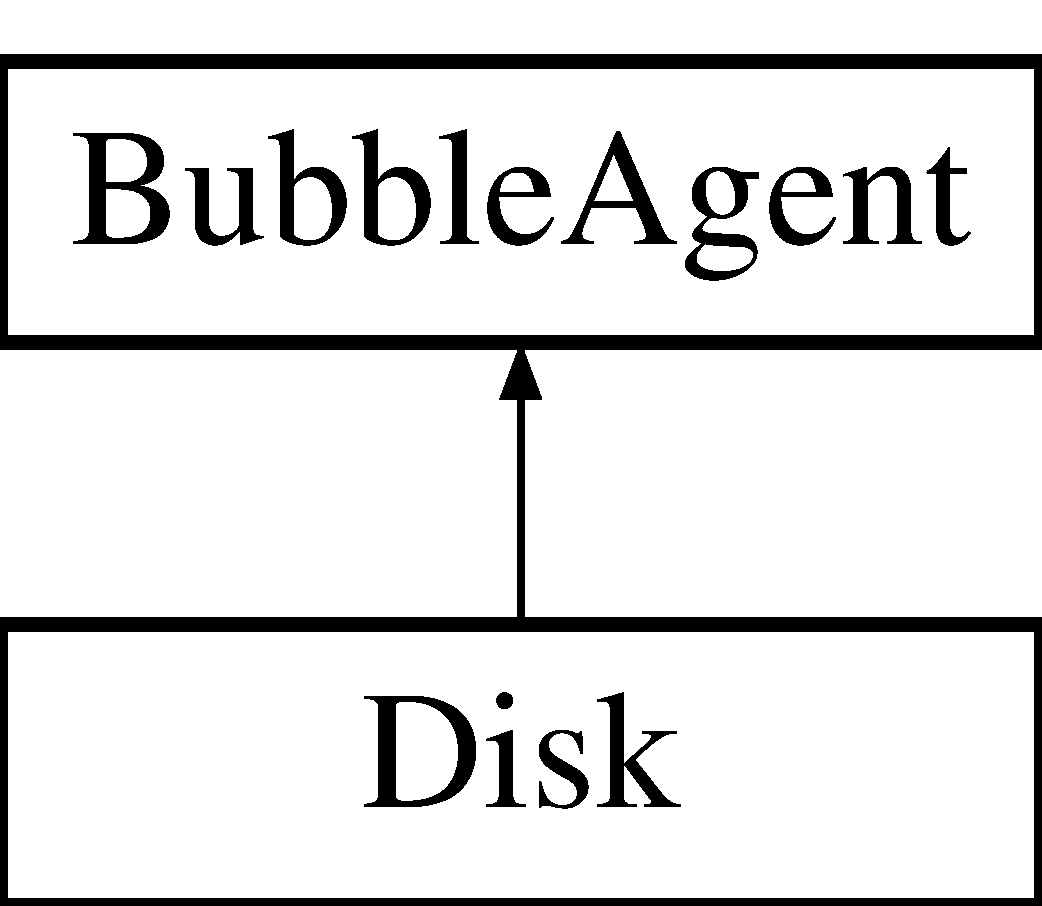
\includegraphics[height=2.000000cm]{class_bubble_agent}
\end{center}
\end{figure}
\subsection*{Public Member Functions}
\begin{DoxyCompactItemize}
\item 
\hypertarget{class_bubble_agent_a2e753e1a4e0e770ee9b3342638c57247}{}{\bfseries Bubble\+Agent} (const Vec3d \&pos)\label{class_bubble_agent_a2e753e1a4e0e770ee9b3342638c57247}

\item 
\hypertarget{class_bubble_agent_aaf7e1faeff29775aed942f4bf1d9fd24}{}Vec3d \& {\bfseries position} ()\label{class_bubble_agent_aaf7e1faeff29775aed942f4bf1d9fd24}

\item 
\hypertarget{class_bubble_agent_ae138dfa99f9da4be1f437820ad947826}{}virtual Vec3d \hyperlink{class_bubble_agent_ae138dfa99f9da4be1f437820ad947826}{get\+\_\+random\+\_\+point} ()=0\label{class_bubble_agent_ae138dfa99f9da4be1f437820ad947826}

\begin{DoxyCompactList}\small\item\em Returns random point on the surface of the agent, which is used as a starting position for a newly created bubble. \end{DoxyCompactList}\end{DoxyCompactItemize}


\subsection{Detailed Description}
Source of bubbles. 

The documentation for this class was generated from the following files\+:\begin{DoxyCompactItemize}
\item 
bubblib/src/bubble\+\_\+agent.\+h\item 
bubblib/src/bubble\+\_\+agent.\+cpp\end{DoxyCompactItemize}

\hypertarget{class_bubble_draw}{}\section{Bubble\+Draw Class Reference}
\label{class_bubble_draw}\index{Bubble\+Draw@{Bubble\+Draw}}
\subsection*{Public Member Functions}
\begin{DoxyCompactItemize}
\item 
\hypertarget{class_bubble_draw_a2ca19c327e25ad0f4ebca0c1fe9b6b4b}{}void {\bfseries create} ()\label{class_bubble_draw_a2ca19c327e25ad0f4ebca0c1fe9b6b4b}

\item 
\hypertarget{class_bubble_draw_a89639f544b3144e2d1a48b36f476410c}{}void {\bfseries destroy} ()\label{class_bubble_draw_a89639f544b3144e2d1a48b36f476410c}

\item 
\hypertarget{class_bubble_draw_ab47721128b96d886f624b0570e3d7305}{}void {\bfseries step\+Sim} ()\label{class_bubble_draw_ab47721128b96d886f624b0570e3d7305}

\item 
\hypertarget{class_bubble_draw_a18520d87ca008ae85ed55bb801e847e8}{}void {\bfseries draw} (\hyperlink{class_shader_program}{Shader\+Program} \&p)\label{class_bubble_draw_a18520d87ca008ae85ed55bb801e847e8}

\end{DoxyCompactItemize}


The documentation for this class was generated from the following files\+:\begin{DoxyCompactItemize}
\item 
preview/src/bubble\+\_\+draw.\+h\item 
preview/src/bubble\+\_\+draw.\+cpp\end{DoxyCompactItemize}

\hypertarget{class_bubble_solver}{}\section{Bubble\+Solver Class Reference}
\label{class_bubble_solver}\index{Bubble\+Solver@{Bubble\+Solver}}


Simulator of dispersed bubble flow.  




{\ttfamily \#include $<$bubble\+\_\+solver.\+h$>$}

\subsection*{Public Member Functions}
\begin{DoxyCompactItemize}
\item 
\hyperlink{class_bubble_solver_a93896970c81c721ee6fbd6989e0090c9}{Bubble\+Solver} (int ni, int nj, int nk, double width\+\_\+x, double scattering\+\_\+freq, double scattering\+\_\+coef, double breakup\+\_\+freq, double scattering\+\_\+impact, double expected\+\_\+radius, double stddev\+\_\+radius, \hyperlink{class_bubble_agent}{Bubble\+Agent} $\ast$agent=nullptr)
\item 
\hyperlink{class_bubble_solver_af0afe26428963124334929d5eadaab37}{Bubble\+Solver} (double wx, double wy, double wz, double dx, \hyperlink{class_bubble_agent}{Bubble\+Agent} $\ast$agent=nullptr)
\begin{DoxyCompactList}\small\item\em Create bubble solver with most parameters being predefined. \end{DoxyCompactList}\item 
\hypertarget{class_bubble_solver_a2f9ca745f73271b0de59936a26450107}{}const std\+::list$<$ \hyperlink{struct_bubble}{Bubble} $>$ \& \hyperlink{class_bubble_solver_a2f9ca745f73271b0de59936a26450107}{get\+\_\+bubbles} () const \label{class_bubble_solver_a2f9ca745f73271b0de59936a26450107}

\begin{DoxyCompactList}\small\item\em Get a list of bubbles. \end{DoxyCompactList}\item 
\hypertarget{class_bubble_solver_a62b6dd926f9000bbe6bfa3cb2f54dd8e}{}double {\bfseries get\+\_\+dx} () const \label{class_bubble_solver_a62b6dd926f9000bbe6bfa3cb2f54dd8e}

\item 
\hypertarget{class_bubble_solver_ae90d580fed7b466e288bcdd5af8a195c}{}int {\bfseries get\+\_\+ni} () const \label{class_bubble_solver_ae90d580fed7b466e288bcdd5af8a195c}

\item 
\hypertarget{class_bubble_solver_aa7e0a2f25e0df0809d89249b90d1041f}{}int {\bfseries get\+\_\+nj} () const \label{class_bubble_solver_aa7e0a2f25e0df0809d89249b90d1041f}

\item 
\hypertarget{class_bubble_solver_abda69fd7367d30f2947fa2741abd81f8}{}int {\bfseries get\+\_\+nk} () const \label{class_bubble_solver_abda69fd7367d30f2947fa2741abd81f8}

\item 
\hypertarget{class_bubble_solver_a1b93d8002f9bda12103fb64b96d66021}{}double {\bfseries scattering\+\_\+freq} () const \label{class_bubble_solver_a1b93d8002f9bda12103fb64b96d66021}

\item 
\hypertarget{class_bubble_solver_ad06bde5694e0c58ee5d76de66d84cb6e}{}double {\bfseries scattering\+\_\+coef} () const \label{class_bubble_solver_ad06bde5694e0c58ee5d76de66d84cb6e}

\item 
\hypertarget{class_bubble_solver_a5d9e60bd12885caa659336dc9e53a826}{}double {\bfseries breakup\+\_\+freq} () const \label{class_bubble_solver_a5d9e60bd12885caa659336dc9e53a826}

\item 
\hypertarget{class_bubble_solver_a6b9bb477ef08fd3c9913acb5e5de23e9}{}double {\bfseries scattering\+\_\+impact} () const \label{class_bubble_solver_a6b9bb477ef08fd3c9913acb5e5de23e9}

\item 
\hypertarget{class_bubble_solver_a011287f768c31ed1ced8651e55c65c40}{}double {\bfseries expected\+\_\+radius} () const \label{class_bubble_solver_a011287f768c31ed1ced8651e55c65c40}

\item 
\hypertarget{class_bubble_solver_a1e00fce9ffd0c16555f51fcf96b34b1b}{}double {\bfseries stddev\+\_\+radius} () const \label{class_bubble_solver_a1e00fce9ffd0c16555f51fcf96b34b1b}

\item 
\hypertarget{class_bubble_solver_a82758ac995f948691a04bfc8e1049dde}{}void {\bfseries scattering\+\_\+freq} (double v)\label{class_bubble_solver_a82758ac995f948691a04bfc8e1049dde}

\item 
\hypertarget{class_bubble_solver_ab8f5d3c4c4bc997a45ae7e5d19995c71}{}void {\bfseries scattering\+\_\+coef} (double v)\label{class_bubble_solver_ab8f5d3c4c4bc997a45ae7e5d19995c71}

\item 
\hypertarget{class_bubble_solver_a0c58fb3970d8863a8aea590ce0318933}{}void {\bfseries breakup\+\_\+freq} (double v)\label{class_bubble_solver_a0c58fb3970d8863a8aea590ce0318933}

\item 
\hypertarget{class_bubble_solver_a771994cbd671af14bb95feb9cfeede52}{}void {\bfseries scattering\+\_\+impact} (double v)\label{class_bubble_solver_a771994cbd671af14bb95feb9cfeede52}

\item 
\hypertarget{class_bubble_solver_ab8b0bb387045922636b27f52d009fa6c}{}void {\bfseries expected\+\_\+radius} (double v)\label{class_bubble_solver_ab8b0bb387045922636b27f52d009fa6c}

\item 
\hypertarget{class_bubble_solver_ae381b289f8f5823ff6286c704fe2cbae}{}void {\bfseries stddev\+\_\+radius} (double v)\label{class_bubble_solver_ae381b289f8f5823ff6286c704fe2cbae}

\item 
\hypertarget{class_bubble_solver_a158c006a1fc29d0332bf50a9a0c6325f}{}void \hyperlink{class_bubble_solver_a158c006a1fc29d0332bf50a9a0c6325f}{advance} (double dt)\label{class_bubble_solver_a158c006a1fc29d0332bf50a9a0c6325f}

\begin{DoxyCompactList}\small\item\em Advance the system by the time dt. \end{DoxyCompactList}\item 
\hypertarget{class_bubble_solver_a02793043b921099423f18ec306f4f8f0}{}void \hyperlink{class_bubble_solver_a02793043b921099423f18ec306f4f8f0}{advance\+\_\+cfl} ()\label{class_bubble_solver_a02793043b921099423f18ec306f4f8f0}

\begin{DoxyCompactList}\small\item\em Advance the system by the maximum timestep allowed by C\+F\+L. \end{DoxyCompactList}\item 
\hypertarget{class_bubble_solver_ad1d5b21ac34864e2056250790d597b72}{}void \hyperlink{class_bubble_solver_ad1d5b21ac34864e2056250790d597b72}{generate\+\_\+n\+\_\+bubbles} (int n)\label{class_bubble_solver_ad1d5b21ac34864e2056250790d597b72}

\begin{DoxyCompactList}\small\item\em Generate n random bubbles on a surface of the agent. \end{DoxyCompactList}\item 
\hypertarget{class_bubble_solver_a0864ddad3a6c432e37197bbfe94f03c0}{}void \hyperlink{class_bubble_solver_a0864ddad3a6c432e37197bbfe94f03c0}{add\+\_\+bubble} (const glm\+::vec3 \&pos, double radius=-\/1.\+0)\label{class_bubble_solver_a0864ddad3a6c432e37197bbfe94f03c0}

\begin{DoxyCompactList}\small\item\em Add a new bubble at a given position of a given radius. If radius isn\textquotesingle{}t specified, it will be set randomly. \end{DoxyCompactList}\item 
\hypertarget{class_bubble_solver_a741e41585765e5924e26e3262edd9b44}{}void \hyperlink{class_bubble_solver_a741e41585765e5924e26e3262edd9b44}{add\+\_\+bubble} (const Vec3d \&pos, double radius=-\/1.\+0)\label{class_bubble_solver_a741e41585765e5924e26e3262edd9b44}

\begin{DoxyCompactList}\small\item\em Add a new bubble at a given position of a given radius. If radius isn\textquotesingle{}t specified, it will be set randomly. \end{DoxyCompactList}\end{DoxyCompactItemize}


\subsection{Detailed Description}
Simulator of dispersed bubble flow. 

Simulator of dispersed bubble flow based on a S\+I\+G\+G\+R\+A\+P\+H 2010 paper \char`\"{}\+A Practical Simulation of Dispersed Bubble Flow\char`\"{} by Doyub Kim, Oh-\/young Song, and Hyeong-\/\+Seok Ko. See the paper for more details. 

\subsection{Constructor \& Destructor Documentation}
\hypertarget{class_bubble_solver_a93896970c81c721ee6fbd6989e0090c9}{}\index{Bubble\+Solver@{Bubble\+Solver}!Bubble\+Solver@{Bubble\+Solver}}
\index{Bubble\+Solver@{Bubble\+Solver}!Bubble\+Solver@{Bubble\+Solver}}
\subsubsection[{Bubble\+Solver}]{\setlength{\rightskip}{0pt plus 5cm}Bubble\+Solver\+::\+Bubble\+Solver (
\begin{DoxyParamCaption}
\item[{int}]{ni, }
\item[{int}]{nj, }
\item[{int}]{nk, }
\item[{double}]{width\+\_\+x, }
\item[{double}]{scattering\+\_\+freq, }
\item[{double}]{scattering\+\_\+coef, }
\item[{double}]{breakup\+\_\+freq, }
\item[{double}]{scattering\+\_\+impact, }
\item[{double}]{expected\+\_\+radius, }
\item[{double}]{stddev\+\_\+radius, }
\item[{{\bf Bubble\+Agent} $\ast$}]{agent = {\ttfamily nullptr}}
\end{DoxyParamCaption}
)}\label{class_bubble_solver_a93896970c81c721ee6fbd6989e0090c9}

\begin{DoxyParams}{Parameters}
{\em ni} & number of cells in X direction \\
\hline
{\em nj} & number of cells in Y direction \\
\hline
{\em nk} & number of cells in Z direction \\
\hline
{\em width\+\_\+x} & length of a container in X direction \\
\hline
{\em scattering\+\_\+freq} & scattering frequency. Characterizes the probabiliy of a given bubble to be scattered. Denoted as nu in the original paper. \\
\hline
{\em scattering\+\_\+coef} & scattering coefficient. Characterizes the the direction of scattering. Denoted as k in the original paper. Should change from -\/1 to 1. \\
\hline
{\em breakup\+\_\+freq} & breakup frequency. Characterizes the expected fraction of bubble to break up at each frame. Denoted as gamma in the original paper. \\
\hline
{\em scattering\+\_\+impact} & scattering impact. This parameter wasn\textquotesingle{}t described in the original paper (in other words, in the original paper it equals one). Setting it greater than one increases the scattering force, making the flow less vertical and more curvy. \\
\hline
{\em expected\+\_\+radius} & whenever new bubble is generated, its radius is set to abs(\+N(mu, sigma)), where N is a normal distribution. This parameter is its mean. \\
\hline
{\em stddev\+\_\+radius} & whenever new bubble is generated, its radius is set to abs(\+N(mu, sigma)), where N is a normal distribution. This parameter is its sigma. \\
\hline
{\em agent} & pointer to a source of bubbles \\
\hline
\end{DoxyParams}
\hypertarget{class_bubble_solver_af0afe26428963124334929d5eadaab37}{}\index{Bubble\+Solver@{Bubble\+Solver}!Bubble\+Solver@{Bubble\+Solver}}
\index{Bubble\+Solver@{Bubble\+Solver}!Bubble\+Solver@{Bubble\+Solver}}
\subsubsection[{Bubble\+Solver}]{\setlength{\rightskip}{0pt plus 5cm}Bubble\+Solver\+::\+Bubble\+Solver (
\begin{DoxyParamCaption}
\item[{double}]{wx, }
\item[{double}]{wy, }
\item[{double}]{wz, }
\item[{double}]{dx, }
\item[{{\bf Bubble\+Agent} $\ast$}]{agent = {\ttfamily nullptr}}
\end{DoxyParamCaption}
)}\label{class_bubble_solver_af0afe26428963124334929d5eadaab37}


Create bubble solver with most parameters being predefined. 


\begin{DoxyParams}{Parameters}
{\em wx} & length of a container in X direction \\
\hline
{\em wy} & length of a container in Y direction \\
\hline
{\em wz} & length of a container in Z direction \\
\hline
{\em dx} & length of a grid cell \\
\hline
{\em agent} & pointer to a source of bubbles \\
\hline
\end{DoxyParams}


The documentation for this class was generated from the following files\+:\begin{DoxyCompactItemize}
\item 
bubblib/src/bubble\+\_\+solver.\+h\item 
bubblib/src/bubble\+\_\+solver.\+cpp\end{DoxyCompactItemize}

\hypertarget{class_disk}{}\section{Disk Class Reference}
\label{class_disk}\index{Disk@{Disk}}


Source of bubbles having a shape of a disk, lying in X\+Z plane.  




{\ttfamily \#include $<$bubble\+\_\+agent.\+h$>$}

Inheritance diagram for Disk\+:\begin{figure}[H]
\begin{center}
\leavevmode
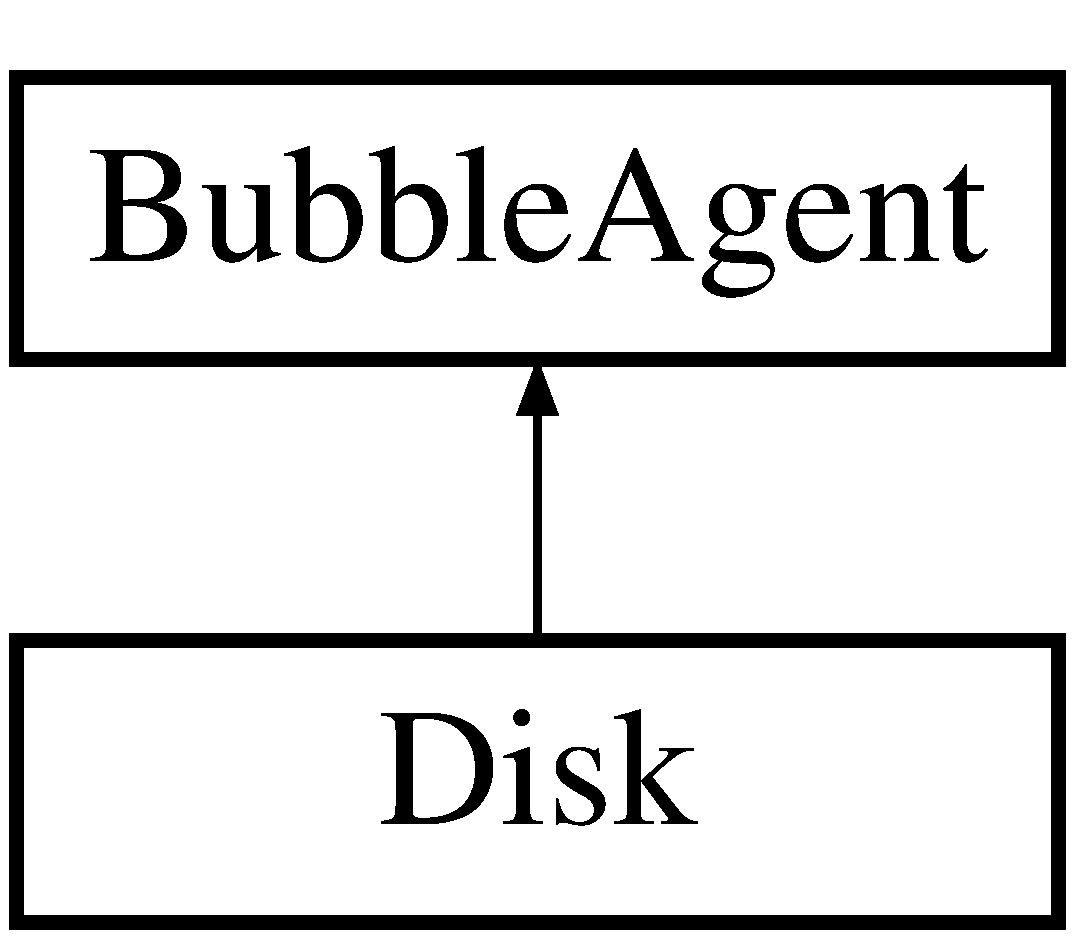
\includegraphics[height=2.000000cm]{class_disk}
\end{center}
\end{figure}
\subsection*{Public Member Functions}
\begin{DoxyCompactItemize}
\item 
\hyperlink{class_disk_a253026ad11118d608e2858c9f63504c6}{Disk} (const Vec3d \&pos, double rad)
\item 
\hypertarget{class_disk_a92d35e24d034a0413dc5a3a25455c7de}{}double \& {\bfseries radius} ()\label{class_disk_a92d35e24d034a0413dc5a3a25455c7de}

\item 
\hypertarget{class_disk_aa1f4238a32897983f6735970a34f8126}{}virtual Vec3d \hyperlink{class_disk_aa1f4238a32897983f6735970a34f8126}{get\+\_\+random\+\_\+point} ()\label{class_disk_aa1f4238a32897983f6735970a34f8126}

\begin{DoxyCompactList}\small\item\em Returns random point on the surface of the agent, which is used as a starting position for a newly created bubble. \end{DoxyCompactList}\end{DoxyCompactItemize}


\subsection{Detailed Description}
Source of bubbles having a shape of a disk, lying in X\+Z plane. 

\subsection{Constructor \& Destructor Documentation}
\hypertarget{class_disk_a253026ad11118d608e2858c9f63504c6}{}\index{Disk@{Disk}!Disk@{Disk}}
\index{Disk@{Disk}!Disk@{Disk}}
\subsubsection[{Disk}]{\setlength{\rightskip}{0pt plus 5cm}Disk\+::\+Disk (
\begin{DoxyParamCaption}
\item[{const Vec3d \&}]{pos, }
\item[{double}]{rad}
\end{DoxyParamCaption}
)\hspace{0.3cm}{\ttfamily [inline]}}\label{class_disk_a253026ad11118d608e2858c9f63504c6}

\begin{DoxyParams}{Parameters}
{\em pos} & center of a disk \\
\hline
{\em rad} & radius of a disk \\
\hline
\end{DoxyParams}


The documentation for this class was generated from the following files\+:\begin{DoxyCompactItemize}
\item 
bubblib/src/bubble\+\_\+agent.\+h\item 
bubblib/src/bubble\+\_\+agent.\+cpp\end{DoxyCompactItemize}

\hypertarget{class_shader_program_1_1_drawable}{}\section{Shader\+Program\+:\+:Drawable Class Reference}
\label{class_shader_program_1_1_drawable}\index{Shader\+Program\+::\+Drawable@{Shader\+Program\+::\+Drawable}}
Inheritance diagram for Shader\+Program\+:\+:Drawable\+:\begin{figure}[H]
\begin{center}
\leavevmode
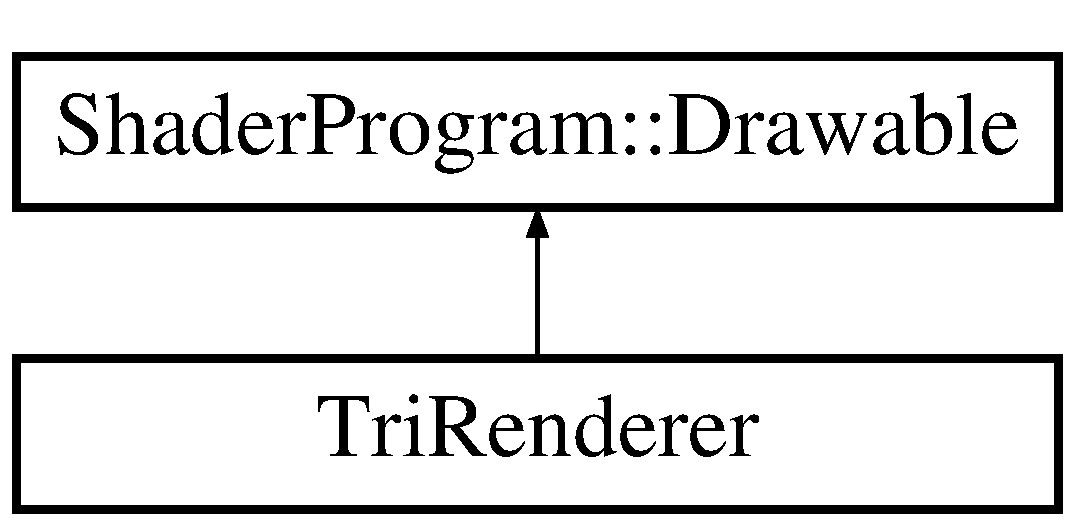
\includegraphics[height=2.000000cm]{class_shader_program_1_1_drawable}
\end{center}
\end{figure}
\subsection*{Public Member Functions}
\begin{DoxyCompactItemize}
\item 
\hypertarget{class_shader_program_1_1_drawable_a332f13c158eea7a688bb82bc38f15c31}{}virtual G\+Lenum {\bfseries draw\+Mode} ()=0\label{class_shader_program_1_1_drawable_a332f13c158eea7a688bb82bc38f15c31}

\item 
\hypertarget{class_shader_program_1_1_drawable_a77ce0c8678c3cf64f3f195e19defb9b6}{}virtual int {\bfseries elem\+Count} ()=0\label{class_shader_program_1_1_drawable_a77ce0c8678c3cf64f3f195e19defb9b6}

\item 
\hypertarget{class_shader_program_1_1_drawable_ac00e86a861a6f0cd4d9f9dd46f77b8e8}{}virtual bool {\bfseries bind\+Idx} ()=0\label{class_shader_program_1_1_drawable_ac00e86a861a6f0cd4d9f9dd46f77b8e8}

\item 
\hypertarget{class_shader_program_1_1_drawable_a16dc86183452514f1597c44fa167f5c6}{}virtual bool {\bfseries bind\+Pos} ()=0\label{class_shader_program_1_1_drawable_a16dc86183452514f1597c44fa167f5c6}

\item 
\hypertarget{class_shader_program_1_1_drawable_aeb05b0e075afe2010bbddfdb3b816f9d}{}virtual bool {\bfseries bind\+Nor} ()=0\label{class_shader_program_1_1_drawable_aeb05b0e075afe2010bbddfdb3b816f9d}

\item 
\hypertarget{class_shader_program_1_1_drawable_a20833f26156ede30f060dee76fbf0c39}{}virtual bool {\bfseries bind\+Col} ()=0\label{class_shader_program_1_1_drawable_a20833f26156ede30f060dee76fbf0c39}

\end{DoxyCompactItemize}


The documentation for this class was generated from the following file\+:\begin{DoxyCompactItemize}
\item 
preview/src/shaderprogram.\+h\end{DoxyCompactItemize}

\hypertarget{class_fluid_sim}{}\section{Fluid\+Sim Class Reference}
\label{class_fluid_sim}\index{Fluid\+Sim@{Fluid\+Sim}}


Grid-\/based fluid solver.  




{\ttfamily \#include $<$fluid\+\_\+sim.\+h$>$}

\subsection*{Public Member Functions}
\begin{DoxyCompactItemize}
\item 
\hyperlink{class_fluid_sim_a2a1b68493a7ad7652c5786dd56400ceb}{Fluid\+Sim} (int n)
\item 
\hyperlink{class_fluid_sim_a77a150bb73bcd7712d99e6f51d6c3f0c}{Fluid\+Sim} (int ni, int nj, int nk, double width\+\_\+x)
\item 
\hypertarget{class_fluid_sim_a571bf8b1dd6172731718e85a39ca1fba}{}double \hyperlink{class_fluid_sim_a571bf8b1dd6172731718e85a39ca1fba}{get\+\_\+u} (int i, int j, int k) const \label{class_fluid_sim_a571bf8b1dd6172731718e85a39ca1fba}

\begin{DoxyCompactList}\small\item\em get u-\/compunent of the fluid velocity at a point (i -\/ 0.\+5, j, k) \end{DoxyCompactList}\item 
\hypertarget{class_fluid_sim_a91ff8cfe3d198bc103564003dc15a862}{}double \hyperlink{class_fluid_sim_a91ff8cfe3d198bc103564003dc15a862}{get\+\_\+v} (int i, int j, int k) const \label{class_fluid_sim_a91ff8cfe3d198bc103564003dc15a862}

\begin{DoxyCompactList}\small\item\em get v-\/compunent of the fluid velocity at a point (i, j -\/ 0.\+5, k) \end{DoxyCompactList}\item 
\hypertarget{class_fluid_sim_a25a82545b4526320c4cd9bb2e8f809e0}{}double \hyperlink{class_fluid_sim_a25a82545b4526320c4cd9bb2e8f809e0}{get\+\_\+w} (int i, int j, int k) const \label{class_fluid_sim_a25a82545b4526320c4cd9bb2e8f809e0}

\begin{DoxyCompactList}\small\item\em get w-\/compunent of the fluid velocity at a point (i, j, k -\/ 0.\+5) \end{DoxyCompactList}\item 
\hypertarget{class_fluid_sim_aca3aeb48eb4c34142c6547fa41525e0f}{}double \hyperlink{class_fluid_sim_aca3aeb48eb4c34142c6547fa41525e0f}{get\+\_\+dx} () const \label{class_fluid_sim_aca3aeb48eb4c34142c6547fa41525e0f}

\begin{DoxyCompactList}\small\item\em get edge length of a grid cell \end{DoxyCompactList}\item 
\hypertarget{class_fluid_sim_ad63a262977c6643ae729cc86ef81bf24}{}int \hyperlink{class_fluid_sim_ad63a262977c6643ae729cc86ef81bf24}{get\+\_\+ni} () const \label{class_fluid_sim_ad63a262977c6643ae729cc86ef81bf24}

\begin{DoxyCompactList}\small\item\em get number of cells in X direction \end{DoxyCompactList}\item 
\hypertarget{class_fluid_sim_a13903a3e84a4efce36157e01ac690a66}{}int \hyperlink{class_fluid_sim_a13903a3e84a4efce36157e01ac690a66}{get\+\_\+nj} () const \label{class_fluid_sim_a13903a3e84a4efce36157e01ac690a66}

\begin{DoxyCompactList}\small\item\em get number of cells in Y direction \end{DoxyCompactList}\item 
\hypertarget{class_fluid_sim_a8135ee3151952a36a0cb3f5b20fcbd50}{}int \hyperlink{class_fluid_sim_a8135ee3151952a36a0cb3f5b20fcbd50}{get\+\_\+nk} () const \label{class_fluid_sim_a8135ee3151952a36a0cb3f5b20fcbd50}

\begin{DoxyCompactList}\small\item\em get number of cells in Z direction \end{DoxyCompactList}\item 
\hypertarget{class_fluid_sim_a7571c38797991175094ada47913917ef}{}void \hyperlink{class_fluid_sim_a7571c38797991175094ada47913917ef}{print} () const \label{class_fluid_sim_a7571c38797991175094ada47913917ef}

\begin{DoxyCompactList}\small\item\em print the state of the tank (i.\+e. velocities, pressure, etc.) \end{DoxyCompactList}\item 
\hypertarget{class_fluid_sim_a08a21095b6ed12a8c610af3b9896781c}{}Array3d \& \hyperlink{class_fluid_sim_a08a21095b6ed12a8c610af3b9896781c}{density} ()\label{class_fluid_sim_a08a21095b6ed12a8c610af3b9896781c}

\begin{DoxyCompactList}\small\item\em grid of density \end{DoxyCompactList}\item 
\hypertarget{class_fluid_sim_a3c657d4e3317ca842c2d9681c85fe365}{}double \& \hyperlink{class_fluid_sim_a3c657d4e3317ca842c2d9681c85fe365}{density} (int i, int j, int k)\label{class_fluid_sim_a3c657d4e3317ca842c2d9681c85fe365}

\begin{DoxyCompactList}\small\item\em density at the center of a cell (i, j, k) \end{DoxyCompactList}\item 
\hypertarget{class_fluid_sim_a62ea50c5c421145e46209b5e7fa8c66e}{}double \hyperlink{class_fluid_sim_a62ea50c5c421145e46209b5e7fa8c66e}{get\+\_\+density} (int i, int j, int k) const \label{class_fluid_sim_a62ea50c5c421145e46209b5e7fa8c66e}

\begin{DoxyCompactList}\small\item\em get density at the center of a cell (i, j, k) \end{DoxyCompactList}\item 
\hypertarget{class_fluid_sim_a034a2c6014c46db41339b8e8d6832958}{}double \hyperlink{class_fluid_sim_a034a2c6014c46db41339b8e8d6832958}{cfl} () const \label{class_fluid_sim_a034a2c6014c46db41339b8e8d6832958}

\begin{DoxyCompactList}\small\item\em maximum allowed time step according to C\+F\+L condition. If it\textquotesingle{}s effectively infinite, 0.\+1 is returned \end{DoxyCompactList}\item 
\hypertarget{class_fluid_sim_a61c83bb89132b4748e353bf90604bafc}{}void \hyperlink{class_fluid_sim_a61c83bb89132b4748e353bf90604bafc}{advance} (double dt)\label{class_fluid_sim_a61c83bb89132b4748e353bf90604bafc}

\begin{DoxyCompactList}\small\item\em advance the fluid by the time step dt. If dt $>$ C\+F\+L(), it will be broken into several smaller steps, each satisfying C\+F\+L \end{DoxyCompactList}\item 
\hypertarget{class_fluid_sim_ad157d29609e7046abfb015f4a69fc207}{}void \hyperlink{class_fluid_sim_ad157d29609e7046abfb015f4a69fc207}{set\+\_\+zero\+\_\+force} ()\label{class_fluid_sim_ad157d29609e7046abfb015f4a69fc207}

\begin{DoxyCompactList}\small\item\em set all external forces to zero \end{DoxyCompactList}\item 
\hypertarget{class_fluid_sim_afd62236b91e338a881475b29de0434de}{}void \hyperlink{class_fluid_sim_afd62236b91e338a881475b29de0434de}{set\+\_\+zero\+\_\+velocity} ()\label{class_fluid_sim_afd62236b91e338a881475b29de0434de}

\begin{DoxyCompactList}\small\item\em set all velocities to zero \end{DoxyCompactList}\item 
\hypertarget{class_fluid_sim_a1f7b3c74cecf8ac32d93f468b6eaef12}{}double \& \hyperlink{class_fluid_sim_a1f7b3c74cecf8ac32d93f468b6eaef12}{force\+\_\+x} (int i, int j, int k)\label{class_fluid_sim_a1f7b3c74cecf8ac32d93f468b6eaef12}

\begin{DoxyCompactList}\small\item\em get X-\/component of an external force, acting at a center of a cell (i, j, k) \end{DoxyCompactList}\item 
\hypertarget{class_fluid_sim_a782b8e8e41e4d5a785188ebb7e2e548c}{}double \& \hyperlink{class_fluid_sim_a782b8e8e41e4d5a785188ebb7e2e548c}{force\+\_\+y} (int i, int j, int k)\label{class_fluid_sim_a782b8e8e41e4d5a785188ebb7e2e548c}

\begin{DoxyCompactList}\small\item\em get Y-\/component of an external force, acting at a center of a cell (i, j, k) \end{DoxyCompactList}\item 
\hypertarget{class_fluid_sim_ad07b83c5ec3f1667091d038dfc1a28a5}{}double \& \hyperlink{class_fluid_sim_ad07b83c5ec3f1667091d038dfc1a28a5}{force\+\_\+z} (int i, int j, int k)\label{class_fluid_sim_ad07b83c5ec3f1667091d038dfc1a28a5}

\begin{DoxyCompactList}\small\item\em get Z-\/component of an external force, acting at a center of a cell (i, j, k) \end{DoxyCompactList}\item 
\hypertarget{class_fluid_sim_a84311b3d42a051b865cf3a0f658275de}{}Vec3d \hyperlink{class_fluid_sim_a84311b3d42a051b865cf3a0f658275de}{get\+\_\+velocity} (const Vec3d \&position) const \label{class_fluid_sim_a84311b3d42a051b865cf3a0f658275de}

\begin{DoxyCompactList}\small\item\em get velocity of a fluid at a given position by interpolating it from grid points \end{DoxyCompactList}\end{DoxyCompactItemize}


\subsection{Detailed Description}
Grid-\/based fluid solver. 

Grid-\/based fluid solver based on Fluid3\+D library by Christopher Batty and a book \char`\"{}\+Fluid Simulation for Computer Graphics\char`\"{} by Robert Bridson. It solves a rectangular tank, full of fluid (no free surface) of varying density. It\textquotesingle{}s assumed that left bottom near corner of the tank is located at (0, 0, 0) 

\subsection{Constructor \& Destructor Documentation}
\hypertarget{class_fluid_sim_a2a1b68493a7ad7652c5786dd56400ceb}{}\index{Fluid\+Sim@{Fluid\+Sim}!Fluid\+Sim@{Fluid\+Sim}}
\index{Fluid\+Sim@{Fluid\+Sim}!Fluid\+Sim@{Fluid\+Sim}}
\subsubsection[{Fluid\+Sim}]{\setlength{\rightskip}{0pt plus 5cm}Fluid\+Sim\+::\+Fluid\+Sim (
\begin{DoxyParamCaption}
\item[{int}]{n}
\end{DoxyParamCaption}
)}\label{class_fluid_sim_a2a1b68493a7ad7652c5786dd56400ceb}

\begin{DoxyParams}{Parameters}
{\em n} & number of cells along each edge of a unit box container \\
\hline
\end{DoxyParams}
\hypertarget{class_fluid_sim_a77a150bb73bcd7712d99e6f51d6c3f0c}{}\index{Fluid\+Sim@{Fluid\+Sim}!Fluid\+Sim@{Fluid\+Sim}}
\index{Fluid\+Sim@{Fluid\+Sim}!Fluid\+Sim@{Fluid\+Sim}}
\subsubsection[{Fluid\+Sim}]{\setlength{\rightskip}{0pt plus 5cm}Fluid\+Sim\+::\+Fluid\+Sim (
\begin{DoxyParamCaption}
\item[{int}]{ni, }
\item[{int}]{nj, }
\item[{int}]{nk, }
\item[{double}]{width\+\_\+x}
\end{DoxyParamCaption}
)}\label{class_fluid_sim_a77a150bb73bcd7712d99e6f51d6c3f0c}

\begin{DoxyParams}{Parameters}
{\em ni} & number of cells in X direction \\
\hline
{\em nj} & number of cells in Y direction \\
\hline
{\em nk} & number of cells in Z direction \\
\hline
{\em width\+\_\+x} & edge length of a grid cell \\
\hline
\end{DoxyParams}


The documentation for this class was generated from the following files\+:\begin{DoxyCompactItemize}
\item 
bubblib/src/fluid\+\_\+sim.\+h\item 
bubblib/src/fluid\+\_\+sim.\+cpp\end{DoxyCompactItemize}

\hypertarget{class_g_l_widget277}{}\section{G\+L\+Widget277 Class Reference}
\label{class_g_l_widget277}\index{G\+L\+Widget277@{G\+L\+Widget277}}
Inheritance diagram for G\+L\+Widget277\+:\begin{figure}[H]
\begin{center}
\leavevmode
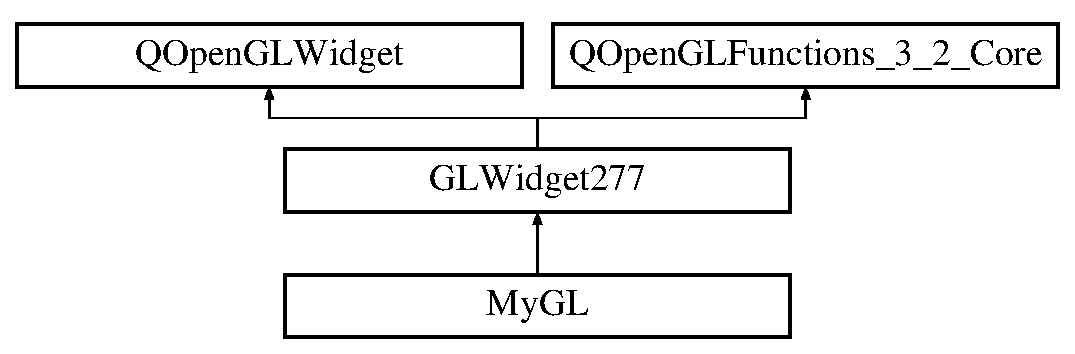
\includegraphics[height=3.000000cm]{class_g_l_widget277}
\end{center}
\end{figure}
\subsection*{Public Member Functions}
\begin{DoxyCompactItemize}
\item 
\hypertarget{class_g_l_widget277_a176b0f695ef85f4c9c77ef0539e307ac}{}{\bfseries G\+L\+Widget277} (Q\+Widget $\ast$parent)\label{class_g_l_widget277_a176b0f695ef85f4c9c77ef0539e307ac}

\item 
\hypertarget{class_g_l_widget277_a2857e8eeef7d84469d423b9363b4f42b}{}void {\bfseries debug\+Context\+Version} ()\label{class_g_l_widget277_a2857e8eeef7d84469d423b9363b4f42b}

\end{DoxyCompactItemize}


The documentation for this class was generated from the following files\+:\begin{DoxyCompactItemize}
\item 
preview/src/glwidget277.\+h\item 
preview/src/glwidget277.\+cpp\end{DoxyCompactItemize}

\hypertarget{class_main_window}{}\section{Main\+Window Class Reference}
\label{class_main_window}\index{Main\+Window@{Main\+Window}}
Inheritance diagram for Main\+Window\+:\begin{figure}[H]
\begin{center}
\leavevmode
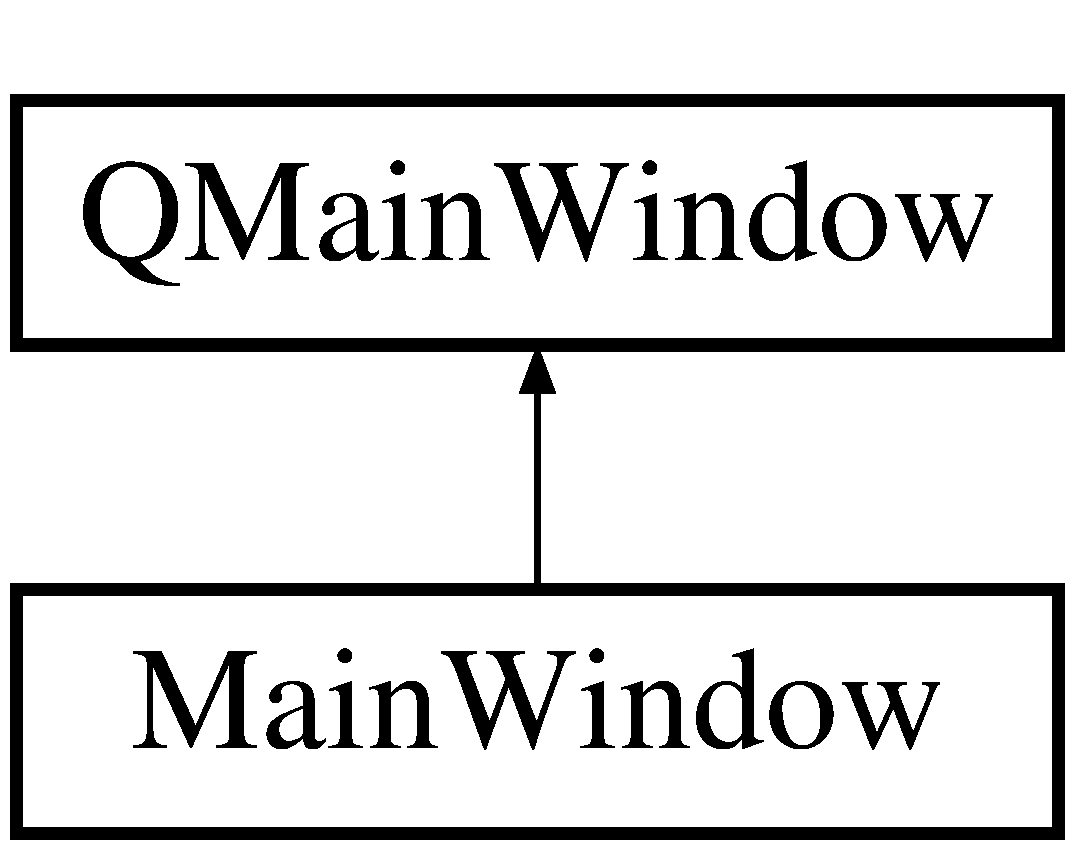
\includegraphics[height=2.000000cm]{class_main_window}
\end{center}
\end{figure}
\subsection*{Public Member Functions}
\begin{DoxyCompactItemize}
\item 
\hypertarget{class_main_window_a8b244be8b7b7db1b08de2a2acb9409db}{}{\bfseries Main\+Window} (Q\+Widget $\ast$parent=0)\label{class_main_window_a8b244be8b7b7db1b08de2a2acb9409db}

\end{DoxyCompactItemize}


The documentation for this class was generated from the following files\+:\begin{DoxyCompactItemize}
\item 
preview/src/mainwindow.\+h\item 
preview/src/mainwindow.\+cpp\end{DoxyCompactItemize}

\hypertarget{class_my_g_l}{}\section{My\+G\+L Class Reference}
\label{class_my_g_l}\index{My\+G\+L@{My\+G\+L}}
Inheritance diagram for My\+G\+L\+:\begin{figure}[H]
\begin{center}
\leavevmode
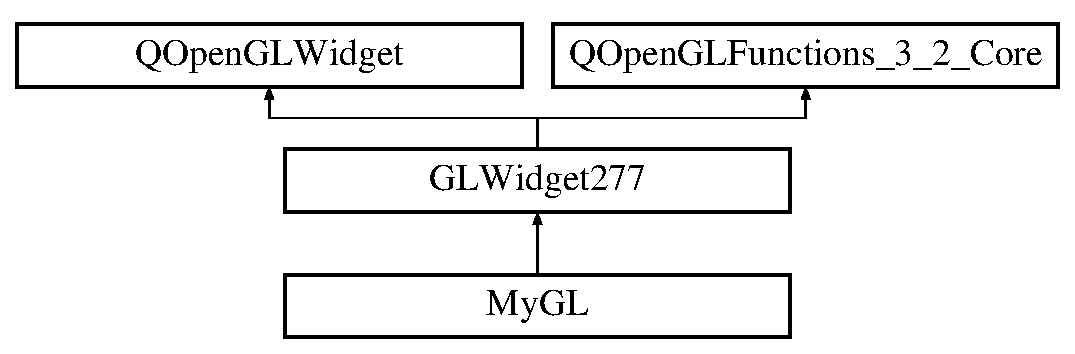
\includegraphics[height=3.000000cm]{class_my_g_l}
\end{center}
\end{figure}
\subsection*{Public Member Functions}
\begin{DoxyCompactItemize}
\item 
\hypertarget{class_my_g_l_a86800be88b23dea695a8b2101d9de2c2}{}{\bfseries My\+G\+L} (Q\+Widget $\ast$parent=0)\label{class_my_g_l_a86800be88b23dea695a8b2101d9de2c2}

\item 
\hypertarget{class_my_g_l_a49ac17e71b1966defbcf305ad2b5f2f0}{}void {\bfseries initialize\+G\+L} ()\label{class_my_g_l_a49ac17e71b1966defbcf305ad2b5f2f0}

\item 
\hypertarget{class_my_g_l_ada6f28601e14f31aae6338aaf1080029}{}void {\bfseries resize\+G\+L} (int, int)\label{class_my_g_l_ada6f28601e14f31aae6338aaf1080029}

\item 
\hypertarget{class_my_g_l_aa3a4e0894b90c26c2c7c0f2d0e191642}{}void {\bfseries paint\+G\+L} ()\label{class_my_g_l_aa3a4e0894b90c26c2c7c0f2d0e191642}

\end{DoxyCompactItemize}
\subsection*{Protected Member Functions}
\begin{DoxyCompactItemize}
\item 
\hypertarget{class_my_g_l_aeedc90ceca802a45f0f1996bf7c41fdf}{}void {\bfseries update\+Camera} ()\label{class_my_g_l_aeedc90ceca802a45f0f1996bf7c41fdf}

\item 
\hypertarget{class_my_g_l_aa8ba50d87d575ba097eba80770790e28}{}void {\bfseries set\+View\+Proj} (const glm\+::mat4 \&viewproj)\label{class_my_g_l_aa8ba50d87d575ba097eba80770790e28}

\item 
\hypertarget{class_my_g_l_aa1630b0a340a088139ffe429b583a993}{}void {\bfseries key\+Press\+Event} (Q\+Key\+Event $\ast$e)\label{class_my_g_l_aa1630b0a340a088139ffe429b583a993}

\item 
\hypertarget{class_my_g_l_aa682b04dfa5fed0e899e9a65dc55a27f}{}void {\bfseries mouse\+Press\+Event} (Q\+Mouse\+Event $\ast$e)\label{class_my_g_l_aa682b04dfa5fed0e899e9a65dc55a27f}

\item 
\hypertarget{class_my_g_l_a55149d95be75efb39706f9ca911b4535}{}void {\bfseries mouse\+Move\+Event} (Q\+Mouse\+Event $\ast$e)\label{class_my_g_l_a55149d95be75efb39706f9ca911b4535}

\item 
\hypertarget{class_my_g_l_ad9606a91a4d893fbfe285e32a1552af8}{}void {\bfseries wheel\+Event} (Q\+Wheel\+Event $\ast$e)\label{class_my_g_l_ad9606a91a4d893fbfe285e32a1552af8}

\end{DoxyCompactItemize}


The documentation for this class was generated from the following files\+:\begin{DoxyCompactItemize}
\item 
preview/src/mygl.\+h\item 
preview/src/mygl.\+cpp\end{DoxyCompactItemize}

\hypertarget{class_shader_program}{}\section{Shader\+Program Class Reference}
\label{class_shader_program}\index{Shader\+Program@{Shader\+Program}}
\subsection*{Classes}
\begin{DoxyCompactItemize}
\item 
class \hyperlink{class_shader_program_1_1_drawable}{Drawable}
\end{DoxyCompactItemize}
\subsection*{Public Member Functions}
\begin{DoxyCompactItemize}
\item 
\hypertarget{class_shader_program_a14461219e634ed659cdb7c049a109eae}{}void {\bfseries create} (const char $\ast$vertfile, const char $\ast$fragfile)\label{class_shader_program_a14461219e634ed659cdb7c049a109eae}

\item 
\hypertarget{class_shader_program_a6b9123f0ce7f9eb5f05ccacbff502553}{}void {\bfseries set\+Model\+Matrix} (const la\+::mat4 \&model)\label{class_shader_program_a6b9123f0ce7f9eb5f05ccacbff502553}

\item 
\hypertarget{class_shader_program_a4ae7594071ac9d9e58ca10b9b9d6fc00}{}void {\bfseries draw} (\hyperlink{class_shader_program_1_1_drawable}{Drawable} \&d)\label{class_shader_program_a4ae7594071ac9d9e58ca10b9b9d6fc00}

\end{DoxyCompactItemize}
\subsection*{Public Attributes}
\begin{DoxyCompactItemize}
\item 
\hypertarget{class_shader_program_a8094baff92b6752e555faf8e2948bdd8}{}Q\+Open\+G\+L\+Shader\+Program {\bfseries prog}\label{class_shader_program_a8094baff92b6752e555faf8e2948bdd8}

\item 
\hypertarget{class_shader_program_a1a272c0832383b6413bf81c076342f4a}{}int {\bfseries attr\+Pos}\label{class_shader_program_a1a272c0832383b6413bf81c076342f4a}

\item 
\hypertarget{class_shader_program_a069fb10108a7a8ca03efa3e3b668662c}{}int {\bfseries attr\+Nor}\label{class_shader_program_a069fb10108a7a8ca03efa3e3b668662c}

\item 
\hypertarget{class_shader_program_afe3f7e1e8b86490c008160b5b5d0d6db}{}int {\bfseries attr\+Col}\label{class_shader_program_afe3f7e1e8b86490c008160b5b5d0d6db}

\item 
\hypertarget{class_shader_program_a2ed5b05aea85814f83a10288267b32d3}{}int {\bfseries unif\+Model}\label{class_shader_program_a2ed5b05aea85814f83a10288267b32d3}

\item 
\hypertarget{class_shader_program_a77e360effc5a2200a7b345690886d263}{}int {\bfseries unif\+Model\+Inv\+Tr}\label{class_shader_program_a77e360effc5a2200a7b345690886d263}

\item 
\hypertarget{class_shader_program_a26586039967a3bb8a9ab06167ae31d14}{}int {\bfseries unif\+View\+Proj}\label{class_shader_program_a26586039967a3bb8a9ab06167ae31d14}

\end{DoxyCompactItemize}


The documentation for this class was generated from the following files\+:\begin{DoxyCompactItemize}
\item 
preview/src/shaderprogram.\+h\item 
preview/src/shaderprogram.\+cpp\end{DoxyCompactItemize}

\hypertarget{class_s_o_p___bubble_streamer}{}\section{S\+O\+P\+\_\+\+Bubble\+Streamer Class Reference}
\label{class_s_o_p___bubble_streamer}\index{S\+O\+P\+\_\+\+Bubble\+Streamer@{S\+O\+P\+\_\+\+Bubble\+Streamer}}


Houdini node Bubble\+Streamer.  




{\ttfamily \#include $<$S\+O\+P\+\_\+\+Bubble\+Streamer.\+h$>$}

Inheritance diagram for S\+O\+P\+\_\+\+Bubble\+Streamer\+:\begin{figure}[H]
\begin{center}
\leavevmode
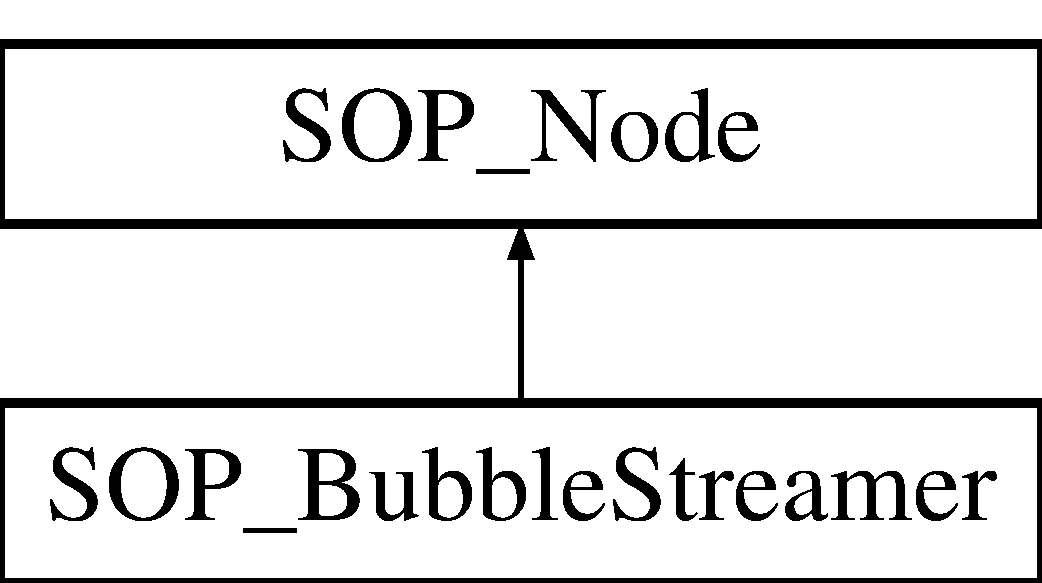
\includegraphics[height=2.000000cm]{class_s_o_p___bubble_streamer}
\end{center}
\end{figure}
\subsection*{Static Public Member Functions}
\begin{DoxyCompactItemize}
\item 
\hypertarget{class_s_o_p___bubble_streamer_a6b0e475f3066f02279547ab0984107c8}{}static O\+P\+\_\+\+Node $\ast$ {\bfseries my\+Constructor} (O\+P\+\_\+\+Network $\ast$, const char $\ast$, O\+P\+\_\+\+Operator $\ast$)\label{class_s_o_p___bubble_streamer_a6b0e475f3066f02279547ab0984107c8}

\end{DoxyCompactItemize}
\subsection*{Static Public Attributes}
\begin{DoxyCompactItemize}
\item 
static P\+R\+M\+\_\+\+Template \hyperlink{class_s_o_p___bubble_streamer_a449d06bab1f64b11f0cfea2565a7ed2a}{my\+Template\+List} \mbox{[}$\,$\mbox{]}
\item 
static C\+H\+\_\+\+Local\+Variable \hyperlink{class_s_o_p___bubble_streamer_a0e2f6d167c4c5622b57ac21ba617fce4}{my\+Variables} \mbox{[}$\,$\mbox{]}
\begin{DoxyCompactList}\small\item\em This optional data stores the list of local variables. \end{DoxyCompactList}\end{DoxyCompactItemize}
\subsection*{Protected Member Functions}
\begin{DoxyCompactItemize}
\item 
\hypertarget{class_s_o_p___bubble_streamer_a81f0643870d928546e0e4cfb76dd27c0}{}{\bfseries S\+O\+P\+\_\+\+Bubble\+Streamer} (O\+P\+\_\+\+Network $\ast$net, const char $\ast$name, O\+P\+\_\+\+Operator $\ast$op)\label{class_s_o_p___bubble_streamer_a81f0643870d928546e0e4cfb76dd27c0}

\item 
\hypertarget{class_s_o_p___bubble_streamer_ab065481deb959e52f6ff28ce479447dc}{}O\+P\+\_\+\+E\+R\+R\+O\+R {\bfseries cook\+Input\+Groups} (O\+P\+\_\+\+Context \&context, int alone)\label{class_s_o_p___bubble_streamer_ab065481deb959e52f6ff28ce479447dc}

\item 
virtual O\+P\+\_\+\+E\+R\+R\+O\+R \hyperlink{class_s_o_p___bubble_streamer_a54fc2a42a26f9fc8ff3ad176a489557a}{cook\+My\+Sop} (O\+P\+\_\+\+Context \&context)
\begin{DoxyCompactList}\small\item\em Disable parameters according to other parameters. \end{DoxyCompactList}\item 
\hypertarget{class_s_o_p___bubble_streamer_a6d8ea032973b1077e81334e193181f13}{}virtual O\+P\+\_\+\+E\+R\+R\+O\+R {\bfseries cook\+My\+Guide1} (O\+P\+\_\+\+Context \&context)\label{class_s_o_p___bubble_streamer_a6d8ea032973b1077e81334e193181f13}

\item 
virtual bool \hyperlink{class_s_o_p___bubble_streamer_a1f67f88545d751c50a581b06cc66605e}{eval\+Variable\+Value} (fpreal \&val, int index, int thread)
\item 
virtual bool \hyperlink{class_s_o_p___bubble_streamer_ab252535c93fb0e1db4cdc2a08dc16228}{eval\+Variable\+Value} (U\+T\+\_\+\+String \&v, int i, int thread)
\end{DoxyCompactItemize}


\subsection{Detailed Description}
Houdini node Bubble\+Streamer. 

This class generates a dispersed bubble flow and imports bubbles to Houdini as particles, allowing user to specify the parameters of the flow 

\subsection{Member Function Documentation}
\hypertarget{class_s_o_p___bubble_streamer_a54fc2a42a26f9fc8ff3ad176a489557a}{}\index{S\+O\+P\+\_\+\+Bubble\+Streamer@{S\+O\+P\+\_\+\+Bubble\+Streamer}!cook\+My\+Sop@{cook\+My\+Sop}}
\index{cook\+My\+Sop@{cook\+My\+Sop}!S\+O\+P\+\_\+\+Bubble\+Streamer@{S\+O\+P\+\_\+\+Bubble\+Streamer}}
\subsubsection[{cook\+My\+Sop}]{\setlength{\rightskip}{0pt plus 5cm}O\+P\+\_\+\+E\+R\+R\+O\+R S\+O\+P\+\_\+\+Bubble\+Streamer\+::cook\+My\+Sop (
\begin{DoxyParamCaption}
\item[{O\+P\+\_\+\+Context \&}]{context}
\end{DoxyParamCaption}
)\hspace{0.3cm}{\ttfamily [protected]}, {\ttfamily [virtual]}}\label{class_s_o_p___bubble_streamer_a54fc2a42a26f9fc8ff3ad176a489557a}


Disable parameters according to other parameters. 

cook\+My\+Sop does the actual work of the S\+O\+P computing, in this case, a L\+S\+Y\+S\+T\+E\+M \hypertarget{class_s_o_p___bubble_streamer_a1f67f88545d751c50a581b06cc66605e}{}\index{S\+O\+P\+\_\+\+Bubble\+Streamer@{S\+O\+P\+\_\+\+Bubble\+Streamer}!eval\+Variable\+Value@{eval\+Variable\+Value}}
\index{eval\+Variable\+Value@{eval\+Variable\+Value}!S\+O\+P\+\_\+\+Bubble\+Streamer@{S\+O\+P\+\_\+\+Bubble\+Streamer}}
\subsubsection[{eval\+Variable\+Value}]{\setlength{\rightskip}{0pt plus 5cm}bool S\+O\+P\+\_\+\+Bubble\+Streamer\+::eval\+Variable\+Value (
\begin{DoxyParamCaption}
\item[{fpreal \&}]{val, }
\item[{int}]{index, }
\item[{int}]{thread}
\end{DoxyParamCaption}
)\hspace{0.3cm}{\ttfamily [protected]}, {\ttfamily [virtual]}}\label{class_s_o_p___bubble_streamer_a1f67f88545d751c50a581b06cc66605e}
This function is used to lookup local variables that you have defined specific to your S\+O\+P. \hypertarget{class_s_o_p___bubble_streamer_ab252535c93fb0e1db4cdc2a08dc16228}{}\index{S\+O\+P\+\_\+\+Bubble\+Streamer@{S\+O\+P\+\_\+\+Bubble\+Streamer}!eval\+Variable\+Value@{eval\+Variable\+Value}}
\index{eval\+Variable\+Value@{eval\+Variable\+Value}!S\+O\+P\+\_\+\+Bubble\+Streamer@{S\+O\+P\+\_\+\+Bubble\+Streamer}}
\subsubsection[{eval\+Variable\+Value}]{\setlength{\rightskip}{0pt plus 5cm}virtual bool S\+O\+P\+\_\+\+Bubble\+Streamer\+::eval\+Variable\+Value (
\begin{DoxyParamCaption}
\item[{U\+T\+\_\+\+String \&}]{v, }
\item[{int}]{i, }
\item[{int}]{thread}
\end{DoxyParamCaption}
)\hspace{0.3cm}{\ttfamily [inline]}, {\ttfamily [protected]}, {\ttfamily [virtual]}}\label{class_s_o_p___bubble_streamer_ab252535c93fb0e1db4cdc2a08dc16228}
Add virtual overload that delegates to the super class to avoid shadow warnings. 

\subsection{Member Data Documentation}
\hypertarget{class_s_o_p___bubble_streamer_a449d06bab1f64b11f0cfea2565a7ed2a}{}\index{S\+O\+P\+\_\+\+Bubble\+Streamer@{S\+O\+P\+\_\+\+Bubble\+Streamer}!my\+Template\+List@{my\+Template\+List}}
\index{my\+Template\+List@{my\+Template\+List}!S\+O\+P\+\_\+\+Bubble\+Streamer@{S\+O\+P\+\_\+\+Bubble\+Streamer}}
\subsubsection[{my\+Template\+List}]{\setlength{\rightskip}{0pt plus 5cm}P\+R\+M\+\_\+\+Template S\+O\+P\+\_\+\+Bubble\+Streamer\+::my\+Template\+List\hspace{0.3cm}{\ttfamily [static]}}\label{class_s_o_p___bubble_streamer_a449d06bab1f64b11f0cfea2565a7ed2a}
{\bfseries Initial value\+:}
\begin{DoxyCode}
= \{
  PRM\_Template(PRM\_STRING, 1, &PRMgroupName, 0, &SOP\_Node::pointGroupMenu,
    0, 0, SOP\_Node::getGroupSelectButton(
    GA\_GROUP\_POINT)),
  PRM\_Template(PRM\_FLT, PRM\_Template::PRM\_EXPORT\_MIN, 1, &nm\_cellsize, &df\_cellsize, 0),
  PRM\_Template(PRM\_FLT, PRM\_Template::PRM\_EXPORT\_MIN, 1, &nm\_simstep, &df\_simstep, 0),
  PRM\_Template(PRM\_FLT, PRM\_Template::PRM\_EXPORT\_MIN, 1, &nm\_scfreq, &df\_scfreq, 0),
  PRM\_Template(PRM\_FLT, PRM\_Template::PRM\_EXPORT\_MIN, 1, &nm\_sccoef, &df\_sccoef, 0),
  PRM\_Template(PRM\_FLT, PRM\_Template::PRM\_EXPORT\_MIN, 1, &nm\_scimpc, &df\_scimpc, 0),
  PRM\_Template(PRM\_FLT, PRM\_Template::PRM\_EXPORT\_MIN, 1, &nm\_brfreq, &df\_brfreq, 0),
  PRM\_Template()
\}
\end{DoxyCode}
Stores the description of the interface of the S\+O\+P in Houdini. Each parm template refers to a parameter. \hypertarget{class_s_o_p___bubble_streamer_a0e2f6d167c4c5622b57ac21ba617fce4}{}\index{S\+O\+P\+\_\+\+Bubble\+Streamer@{S\+O\+P\+\_\+\+Bubble\+Streamer}!my\+Variables@{my\+Variables}}
\index{my\+Variables@{my\+Variables}!S\+O\+P\+\_\+\+Bubble\+Streamer@{S\+O\+P\+\_\+\+Bubble\+Streamer}}
\subsubsection[{my\+Variables}]{\setlength{\rightskip}{0pt plus 5cm}C\+H\+\_\+\+Local\+Variable S\+O\+P\+\_\+\+Bubble\+Streamer\+::my\+Variables\hspace{0.3cm}{\ttfamily [static]}}\label{class_s_o_p___bubble_streamer_a0e2f6d167c4c5622b57ac21ba617fce4}
{\bfseries Initial value\+:}
\begin{DoxyCode}
= \{
  
  
  \{ 0, 0, 0 \},
\}
\end{DoxyCode}


This optional data stores the list of local variables. 



The documentation for this class was generated from the following files\+:\begin{DoxyCompactItemize}
\item 
hplugin/src/S\+O\+P\+\_\+\+Bubble\+Streamer.\+h\item 
hplugin/src/S\+O\+P\+\_\+\+Bubble\+Streamer.\+cpp\end{DoxyCompactItemize}

\hypertarget{class_tri_renderer}{}\section{Tri\+Renderer Class Reference}
\label{class_tri_renderer}\index{Tri\+Renderer@{Tri\+Renderer}}
Inheritance diagram for Tri\+Renderer\+:\begin{figure}[H]
\begin{center}
\leavevmode
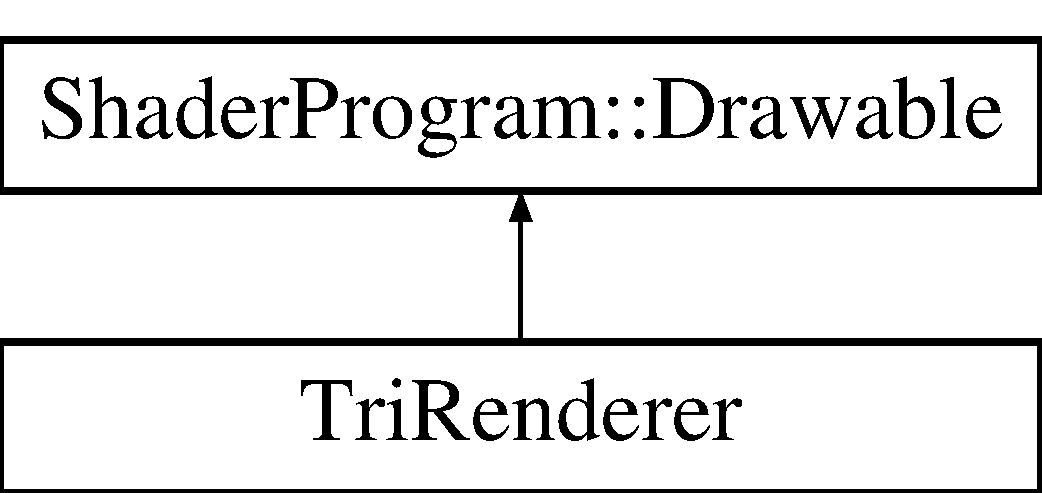
\includegraphics[height=2.000000cm]{class_tri_renderer}
\end{center}
\end{figure}
\subsection*{Public Member Functions}
\begin{DoxyCompactItemize}
\item 
\hypertarget{class_tri_renderer_a8c41a491f72487c146a25cd9b239ede5}{}void {\bfseries create} ()\label{class_tri_renderer_a8c41a491f72487c146a25cd9b239ede5}

\item 
\hypertarget{class_tri_renderer_a07cc288b5d04572f1f784b14ce7f3c17}{}void {\bfseries destroy} ()\label{class_tri_renderer_a07cc288b5d04572f1f784b14ce7f3c17}

\item 
\hypertarget{class_tri_renderer_a1e77e021d03ee3c3704e7c1934a54619}{}void {\bfseries replace\+Mesh} (const std\+::vector$<$ \hyperlink{structvec3tri}{vec3tri} $>$ \&pos)\label{class_tri_renderer_a1e77e021d03ee3c3704e7c1934a54619}

\item 
\hypertarget{class_tri_renderer_a9eecf387616bc70eeb24f0b56cc0564e}{}G\+Lenum {\bfseries draw\+Mode} ()\label{class_tri_renderer_a9eecf387616bc70eeb24f0b56cc0564e}

\item 
\hypertarget{class_tri_renderer_a82d0b59bb47be528c49bf13cdfe6a02e}{}int {\bfseries elem\+Count} ()\label{class_tri_renderer_a82d0b59bb47be528c49bf13cdfe6a02e}

\item 
\hypertarget{class_tri_renderer_ae42558e906dca14cc6a2c3af0186a8a2}{}bool {\bfseries bind\+Idx} ()\label{class_tri_renderer_ae42558e906dca14cc6a2c3af0186a8a2}

\item 
\hypertarget{class_tri_renderer_a1dc7908d880dd63e1ff8121865b8f74d}{}bool {\bfseries bind\+Pos} ()\label{class_tri_renderer_a1dc7908d880dd63e1ff8121865b8f74d}

\item 
\hypertarget{class_tri_renderer_ac0a43cd55c2a5a96762b751fa10cac91}{}bool {\bfseries bind\+Nor} ()\label{class_tri_renderer_ac0a43cd55c2a5a96762b751fa10cac91}

\item 
\hypertarget{class_tri_renderer_a1f74aaf83576b14d1812e04b8d60ec97}{}bool {\bfseries bind\+Col} ()\label{class_tri_renderer_a1f74aaf83576b14d1812e04b8d60ec97}

\end{DoxyCompactItemize}


The documentation for this class was generated from the following files\+:\begin{DoxyCompactItemize}
\item 
preview/src/trirenderer.\+h\item 
preview/src/trirenderer.\+cpp\end{DoxyCompactItemize}

\hypertarget{structuint3}{}\section{uint3 Struct Reference}
\label{structuint3}\index{uint3@{uint3}}
\subsection*{Public Attributes}
\begin{DoxyCompactItemize}
\item 
\hypertarget{structuint3_ad39b53a9e887b32825653ebc69600c39}{}G\+Luint {\bfseries a}\label{structuint3_ad39b53a9e887b32825653ebc69600c39}

\item 
\hypertarget{structuint3_a0142d6201386e26b810a573b0398114c}{}G\+Luint {\bfseries b}\label{structuint3_a0142d6201386e26b810a573b0398114c}

\item 
\hypertarget{structuint3_aa5ca4d25316a3c093dd052048ff10f89}{}G\+Luint {\bfseries c}\label{structuint3_aa5ca4d25316a3c093dd052048ff10f89}

\end{DoxyCompactItemize}


The documentation for this struct was generated from the following file\+:\begin{DoxyCompactItemize}
\item 
preview/src/trirenderer.\+h\end{DoxyCompactItemize}

\hypertarget{structvec3tri}{}\section{vec3tri Struct Reference}
\label{structvec3tri}\index{vec3tri@{vec3tri}}
\subsection*{Public Attributes}
\begin{DoxyCompactItemize}
\item 
\hypertarget{structvec3tri_abbce1765e745050a6e708bb848b28492}{}glm\+::vec3 {\bfseries a}\label{structvec3tri_abbce1765e745050a6e708bb848b28492}

\item 
\hypertarget{structvec3tri_a3c1a84a5f66c500026552c13a4d2b7f3}{}glm\+::vec3 {\bfseries b}\label{structvec3tri_a3c1a84a5f66c500026552c13a4d2b7f3}

\item 
\hypertarget{structvec3tri_a9307252444ab03989eca2857c4f29c73}{}glm\+::vec3 {\bfseries c}\label{structvec3tri_a9307252444ab03989eca2857c4f29c73}

\end{DoxyCompactItemize}


The documentation for this struct was generated from the following file\+:\begin{DoxyCompactItemize}
\item 
preview/src/trirenderer.\+h\end{DoxyCompactItemize}

%--- End generated contents ---

% Index
\backmatter
\newpage
\phantomsection
\clearemptydoublepage
\addcontentsline{toc}{chapter}{Index}
\printindex

\end{document}
